%!TEX root = report.tex
\subsection{Arrival}
\par This endpoint serves as a wrapper for the \acrshort{tfl} Live Bus API endpoint. Given a set of \acrshort{gps} coordinates and the radius of circle, this API endpoint returns the arrival times of buses arriving at stops within the circle.

\subsubsection{Query URL \& Parameters}
\par The base URL for this endpoint is \url{http://delay.doc.ic.ac.uk:5000/arrivals/?}. The required parameters include the latitude and the longitude of the \acrshort{gps} coordinates, and the radius in meters. An example query URL would be \url{http://delay.doc.ic.ac.uk:5000/arrivals/?latitude=51.495171603309615&longitude=-0.1883983612060547&radius=100}.

\subsubsection{Result Format}
\par The query result is a list of bus stops within the circle. Each bus stop entry has basic information about the stop, and a list of the buses arriving at the stop in the next 30 minutes, grouped by the bus routes. Within each route, the \texttt{estimatedTimeInSeconds} shows the arrival times of the buses arriving at the given stop. See Figure \ref{fig:arrival_api} for example response.


\begin{figure}
\centering
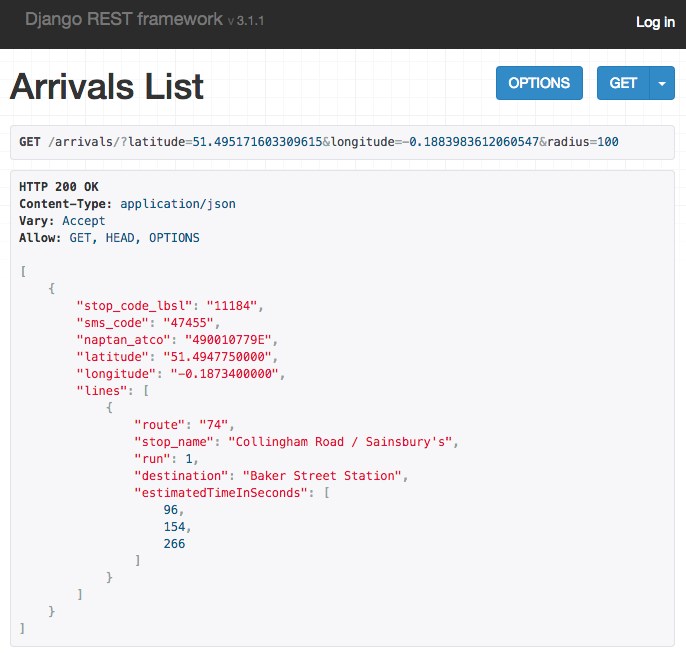
\includegraphics[width=\textwidth]{figures/arrival_api.png}
\caption{\label{fig:arrival_api} Sample Response for Arrivals API}
\end{figure}

\section{Summary of Data Service API}
\par These three \acrshort{api} endpoints provide easy access to the reference, current, and historical timetables produced. Other developers can use the data to produce bus delay predictions or build software applications for London bus passengers. We evaluated the accuracy of the timetables and the performance of the \acrshort{api} in Chapter \ref{ch:evaluation}.
